
% $Header: /cvsroot/latex-beamer/latex-beamer/solutions/generic-talks/generic-ornate-15min-45min.en.tex,v 1.5 2007/01/28 20:48:23 tantau Exp $

\documentclass[smaller]{beamer}
\mode<presentation>
{
  \usetheme{Singapore}
  \usefonttheme[onlymath]{serif}
  % or ...
 %  \setbeamercovered{transparent}
  % or whatever (possibly just delete it)
}

\usepackage{textcomp}
\usepackage[czech]{babel}
% or whatever
\usepackage[utf8]{inputenc}
% or whatever
%\usepackage{times}
%\usepackage[T1]{fontenc}
% Or whatever. Note that the encoding and the font should match. If T1
% does not look nice, try deleting the line with the fontenc.


\title{PAS07 -- Interval estimates and auxiliary distributions}

\author{Jan B\v rezina}
\institute % (optional, but mostly needed)
{
  %\inst{2}%
  Technical University of Liberec
}


% If you wish to uncover everything in a step-wise fashion, uncomment
% the following command: 

%\beamerdefaultoverlayspecification{<+->}

% ***************************************** SYMBOLS
\def\div{{\rm div}}
\def\Lapl{\Delta}
\def\grad{\nabla}
\def\supp{{\rm supp}}
\def\dist{{\rm dist}}
%\def\chset{\mathbbm{1}}
\def\chset{1}

\def\Tr{{\rm Tr}}
\def\sgn{{\rm sgn}}
\def\to{\rightarrow}
\def\weakto{\rightharpoonup}
\def\imbed{\hookrightarrow}
\def\cimbed{\subset\subset}
\def\range{{\mathcal R}}
\def\leprox{\lesssim}
\def\argdot{{\hspace{0.18em}\cdot\hspace{0.18em}}}
\def\Distr{{\mathcal D}}
\def\calK{{\mathcal K}}
\def\FromTo{|\rightarrow}
\def\convol{\star}
\def\impl{\Rightarrow}
\DeclareMathOperator*{\esslim}{esslim}
\DeclareMathOperator*{\esssup}{ess\,sup}
\DeclareMathOperator{\ess}{ess}
\DeclareMathOperator{\osc}{osc}
\DeclareMathOperator{\curl}{curl}

%\def\Ess{{\rm ess}}
%\def\Exp{{\rm exp}}
%\def\Implies{\Longrightarrow}
%\def\Equiv{\Longleftrightarrow}
% ****************************************** GENERAL MATH NOTATION
\def\Real{{\rm\bf R}}
\def\Rd{{{\rm\bf R}^{\rm 3}}}
\def\RN{{{\rm\bf R}^N}}
\def\D{{\mathbb D}}
\def\Nnum{{\mathbb N}}
\def\Measures{{\mathcal M}}
\def\d{\,{\rm d}}               % differential
\def\sdodt{\genfrac{}{}{}{1}{\rm d}{{\rm d}t}}
\def\dodt{\genfrac{}{}{}{}{\rm d}{{\rm d}t}}

\def\vc#1{\mathbf{\boldsymbol{#1}}}     % vector
\def\tn#1{{\mathbb{#1}}}    % tensor
\def\abs#1{\lvert#1\rvert}
\def\Abs#1{\bigl\lvert#1\bigr\rvert}
\def\bigabs#1{\bigl\lvert#1\bigr\rvert}
\def\Bigabs#1{\Big\lvert#1\Big\rvert}
\def\ABS#1{\left\lvert#1\right\rvert}
\def\norm#1{\bigl\Vert#1\bigr\Vert} %norm
\def\close#1{\overline{#1}}
\def\inter#1{#1^\circ}
\def\ol#1{\overline{#1}}
\def\ul#1{\underline{#1}}
\def\eqdef{\mathrel{\mathop:}=}     % defining equivalence
\def\where{\,|\,}                    % "where" separator in set's defs
\def\timeD#1{\dot{\overline{{#1}}}}

% ******************************************* USEFULL MACROS
\def\RomanEnum{\renewcommand{\labelenumi}{\rm (\roman{enumi})}}   % enumerate by roman numbers
\def\rf#1{(\ref{#1})}                                             % ref. shortcut
\def\prtl{\partial}                                        % partial deriv.
\def\Names#1{{\scshape #1}}
\def\rem#1{{\parskip=0cm\par!! {\sl\small #1} !!}}

\def\Xint#1{\mathchoice
{\XXint\displaystyle\textstyle{#1}}%
{\XXint\textstyle\scriptstyle{#1}}%
{\XXint\scriptstyle\scriptscriptstyle{#1}}%
{\XXint\scriptscriptstyle\scriptscriptstyle{#1}}%
\!\int}
\def\XXint#1#2#3{{\setbox0=\hbox{$#1{#2#3}{\int}$}
\vcenter{\hbox{$#2#3$}}\kern-.5\wd0}}
\def\ddashint{\Xint=}
\def\dashint{\Xint-}

% ******************************************* DOCUMENT NOTATIONS
% document specific
\def\rh{\varrho}
\def\vl{{\vc{u}}}
\def\th{\vartheta}
\def\vx{\vc{x}}
\def\vX{\vc{X}}
\def\vr{\vc{r}}
\def\veta{\vc{\eta}}
\def\dx{\,\d\vx}
\def\dt{\,\d t}
\def\bulk{\zeta}
\def\cS{\close{S}}
\def\eps{\varepsilon}
\def\phi{\varphi}
\def\Bog{{\mathcal B}}
\def\Riesz{{\mathcal R}}
\def\distr{\mathcal D}
\def\Item{$\bullet$}

\def\MEtst{\mathcal T}
%***************************************************************************
\setbeamercolor{my blue}{fg=blue}
\def\blue#1{{\usebeamercolor[fg]{my blue} #1}}

\setbeamercolor{my green}{fg=green}
\def\green#1{{\usebeamercolor[fg]{my green} #1}}

% color for term definition
\setbeamercolor{my orange}{fg=orange}
\def\df#1{{\usebeamercolor[fg]{my orange} #1}}
\def\xskip{{\vspace{2ex}}}

\def\cz#1{{\small (#1)}}

\def\E{\vc{\mathsf{E}}}

\begin{document}

\begin{frame}
  \titlepage
\end{frame}

\begin{frame}{Motivation example}
  Concentration of an ingredient in a solution has been measured on 50 samples giving an average concentration $19.7$
  and standard deviation $0.255$. 
  \begin{enumerate}
   \item  Determine a two-side interval $(c_b, c_t)$ (confidence interval) for the true concentration in the solution, so that 
          true concentration is contained with probability $95\%$.
   \item  Determine lower estimate of the concentration $C_b$, such that true concentration is grater with probability  $95\%$.
   \item  Determine value $x$ so that we can say: ``Concentration is smaller then $x$ with probability $95\%$.''
   \end{enumerate}
\end{frame}

\begin{frame}{Transformation of normal distributed variable}
\begin{enumerate}
 \item general normally distributed random variable 
  \[ X \sim N(\mu, \sigma^2)\]
 \item sum of $n$ independent variables with same normal distributions
  \[ \sum_i X_i \sim N(n \mu, n \sigma^2)\]
% proved best with characteristic functions

 \item sample average of the same random vector
  \[ \ol{X} \sim N(\mu, \sigma^2 / n)\]
 \item shifted average
  \[ \ol{X} - \mu \sim N(0, ( \sigma / \sqrt(n) ) ^2 )\] 
 \item standartized average
  \[ Z=\frac{\ol{X} - \mu}{\sigma} \sqrt{n} \sim N(0, 1)\]
\end{enumerate}

\end{frame}

\begin{frame}{derivation of Two-side estimate}
Consider symmetric probabilities of error tails, $u_\alpha$ is quantile of standard normal distribution:
\[
  P( Z < u_{0.025}) = 0.025 \quad \& \quad P( Z > u_{1-0.025}) = 0.025 = \frac{\alpha}{2}
\]
\[
 P( u_{0.025} < Z < u_{1- 0.025} ) = 0.95 = 1-\alpha
\]
\[
 P( -u_{1-\frac{\alpha}{2}} < \frac{\ol{X} - \mu}{\sigma}\sqrt{n} < u_{1-\frac{\alpha}{2}} ) = 1-\alpha
\]
\[
 P( \ol{X} - \frac{\sigma }{\sqrt{n}}u_{1-\frac{\alpha}{2}} < \mu < \ol{X} + \frac{\sigma }{\sqrt{n}}u_{1-\frac{\alpha}{2}} ) = 1-\alpha
\]
\end{frame}




\begin{frame}{Back to the example}
We approximate unknown $\sigma$ by sample deviation, since $n$ is big enough $n>30$, and $\alpha$ is modest.
\[
  \ol{X} = 19.7, \qquad \sigma \approx S =  0.255, \qquad n=50, \qquad \alpha=0.05,\qquad  u_{0.975} = 1.96
\]

\[
  c_b = \ol{X} - \frac{\sigma u_{1-\frac{\alpha}{2}}}{\sqrt{n}} = 19.63
\]

\[
  c_t = \ol{X} + \frac{\sigma u_{1-\frac{\alpha}{2}}}{\sqrt{n}} = 19.77
\]

\[
  C_b = \ol{X} - \frac{\sigma u_{1-\alpha}}{\sqrt{n}} = 19.64
\]

\[
  x= C_t = \ol{X} + \frac{\sigma u_{1-\alpha}}{\sqrt{n}} = 19.76
\]


\end{frame}
  
  
\begin{frame}[fragile]{Interval estimate for $\mu$ with unknown $\sigma$}
 We replace $\sigma$ by sample standard deviation $S_n$. What is true distribution of variable 
 \[
    Z_n = \frac{\ol{X} - \mu}{S_n} \sqrt{n}, \qquad S_n^2=\frac{1}{n-1} \sum_i (X_i - \ol{X})^2
 \]
 \df{Student's distribution} with $n-1$ degrees of freedom - $t_{n-1}$.
 
 \xskip
 \verb#> x=seq(-4,4,0.01)#\\
 \verb#> plot(x, dnorm(x), type='l')#\\
 \verb#> lines( x, dt(x, df=5))#
\end{frame}	

\begin{frame}{Student's t-distribution}
 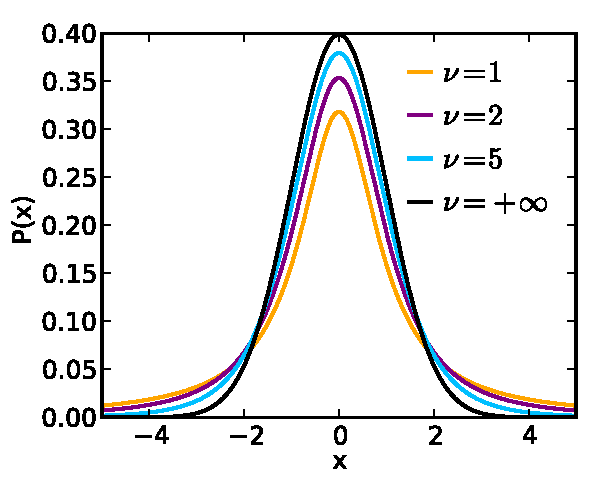
\includegraphics[scale=0.8]{07_Student_t.pdf}
\end{frame}


\begin{frame}{Interval estimate for $\mu$ with unknown $\sigma$}

two-side confidence interval
\[
 P\left\{ \ol{X} - \frac{S_n}{\sqrt{n}}t_{n-1}(1-\alpha/2) < \mu < \ol{X} + \frac{S_n}{\sqrt{n}}t_{n-1}(1-\alpha/2) \right\} = 1-\alpha
\]
left one-side interval estimate
\[
 P\left\{ \ol{X} - \frac{S_n}{\sqrt{n}}t_{n-1}(1-\alpha) < \mu \right\} = 1-\alpha
\]
right one-side interval estimate
\[
 P\left\{ \mu < \ol{X} + \frac{S_n}{\sqrt{n}}t_{n-1}(1-\alpha) \right\} = 1-\alpha
\]
    
\end{frame}
  
  
\begin{frame}{Number of customers in hypermarket}
A hypermarket is interested in the number of customers at Friday afternoon (noon - 6 pm). 
A study gives following numbers: 3756, 2987, 3042, 4206, 3597 (for 5 consecutive Fridays).
Determine two-side and one-side interval estimates.

\xskip
\dots Litschmanová, p. 240
\end{frame}


\begin{frame}{Interval estimate for variance}
  
\dots Litschmanová, p. 241  

\xskip
\blue{$\chi^2$-distribution}
\end{frame}
  
\begin{frame}{Chi-squared distribution}
 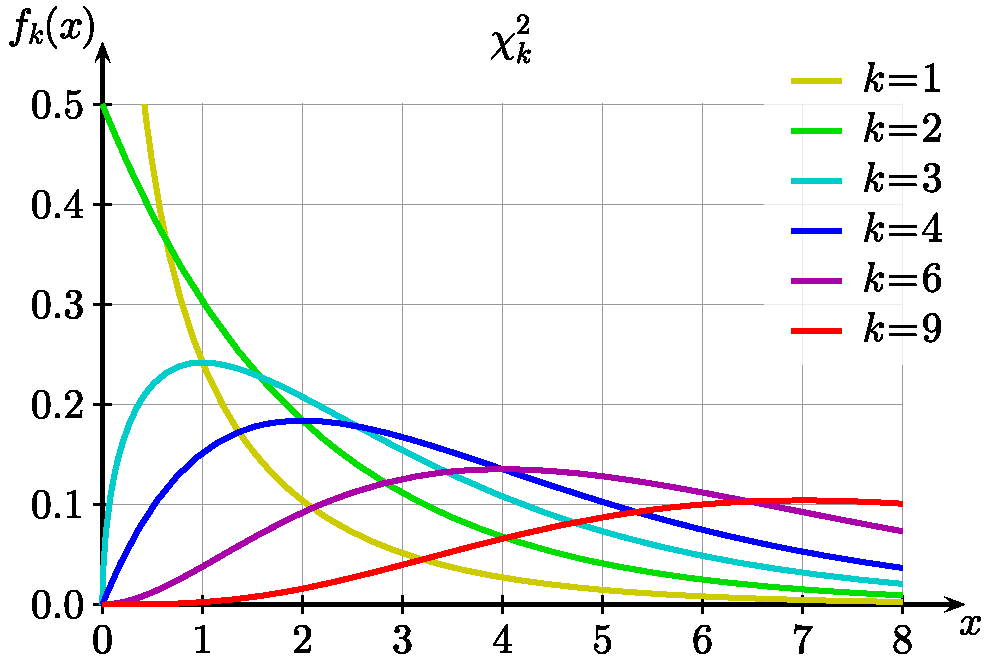
\includegraphics[scale=0.5]{07_Chi-square.pdf}
\end{frame}

  
\begin{frame}{Interval estimate for relative frequency}
We have data $\{X_i\}$ z $Alt(\pi)$. Sample relative freq. is $p$.
Using Moivre-Laplace theorem:
\[
U = \frac{p - \pi}{\sqrt{\pi(1-\pi}}\sqrt{n} \quad \sim N(0,1)
\]
Tedy 
\[
 P\big(u(\alpha/2) \le U \le u(1-\alpha/2)\big) = 1-\alpha
\]
po upravě:
\[
 P\big(p-\Delta < \pi < p+\Delta) = 1-\alpha
\]
\[
 \Delta = \sqrt{\frac{\pi(1-\pi)}{n}}u(1-\alpha/2) \pause \approx \sqrt{\frac{p(1-p)}{n}}u(1-\alpha/2)
\]

\dots Litschmanová, p. 244
\end{frame}
  
  
\begin{frame}{Size of sample}
\dots  Litschmanová, p. 246
\end{frame}
  

\end{document}


